\documentclass[12pt]{article}
\usepackage[utf8]{inputenc}
\usepackage{amsmath,amsfonts}
\usepackage{hyperref}
\usepackage{tikz}
\usepackage{pgfplots}
\usepackage{xcolor}
\usepackage[left=2cm,right=2cm,top=3cm,bottom=3cm,footskip=0cm,foot=1cm,marginparsep=0cm,marginparwidth=1cm,headsep=0.5cm,headheight=1cm]{geometry}

\definecolor{myblue}{rgb}{0.00,0.39,0.67}
\definecolor{myred}{rgb}{0.86,0.08,0.14}
\definecolor{mygreen}{rgb}{0.07,0.52,0.07}
\definecolor{myorange}{rgb}{0.99,0.32,0.08}
\definecolor{mygray}{rgb}{0.5,0.5,0.5}


\def\Ef{\eta}
\def\happy{\mathcal{H}}
\def\gym{\mathcal{G}}
\def\bonus{\mathcal{B}}

\def\Sc{S_\text{c}}
\def\Si{S_\text{i}}
\def\Sf{S_\text{f}}
\def\Ec{E_\text{c}}

\title{Battle stats formula}
\author{Kivou [2000607]}

\begin{document}
\maketitle
\par {\it Starting from a formula that gives the battle stats gains for a certain amount of energy, we derive here  a formula that gives the battle stats as a function of energy and, in turns, the energy needed to reach a certain battle stats level from a given one.}

\section{Theory}
\subsection{Gym gain formula}
\href{https://www.torn.com/forums.php?p=threads&f=61&t=16003284&b=0&a=0&start=0&to=17684755}{Vladar [1996140]} gives a formula defining the battle stats gains as a function of the current stat, the energy spent on train and other parameters.

\par In this formula and for the rest we will need:
\begin{itemize}
    \item 2 variables and their differentials
    \begin{itemize}
        \item Energy $E$ and $dE$
        \item Battle stats $S$ and $dS$
    \end{itemize}
    \item 6 known coefficients
        \begin{itemize}
            \item $a = 0.0000003480061091$
            \item $b = 250$
            \item $c = 0.000003091619094$
            \item $d = 0.0000682775184551527$
            \item $e = -0.0301431777$
            \item $\Sc = 50\,000\,000$ (known as the battle stats cap)
        \end{itemize}
    \item 3 states variables
    \begin{itemize}
        \item Happy level $\happy$
        \item Gym coefficient $\gym$
        \item Gym gain bonus $\bonus$
    \end{itemize}
\end{itemize}

The Vladar formula eq.\eqref{eq:valdar} gives the stats gains $dS$ as a function of the current stats $S$ and the energy spent $dE$. It is usually written:
\begin{equation}
    dS = \left[ (a\ln(\happy+b)+c) \bar{S} + d(\happy+b) + e \right](1+\bonus)\gym dE
    \label{eq:valdar}
\end{equation}
with $\bar{S} = \min(\Sc, S)$

\par By introducing 2 new parameters $\alpha$ and $\beta$ that depend only on the 5 coefficients $a, b, c, d, e$ and the state variables $\happy, \bonus, \gym$, eq.\eqref{eq:valdar} can be written as follow:
\begin{equation}
    \frac{dS}{dE} = \alpha \bar{S} + \beta \quad \Leftrightarrow \quad \frac{dS}{dE} - \alpha \bar{S} = \beta
    \label{eq:valdar-diff}
\end{equation}
with
\begin{equation}
    \left\{\begin{aligned}
        \alpha &= (a\ln(\happy+b)+c)(1+\bonus)\gym\\
        \beta &= (d(\happy+b) +e)(1+\bonus)\gym
    \end{aligned}\right.
\end{equation}
From now on we assume that $\alpha > 0$ and $\beta > 0$.

\subsection{Battle stats formula}
\par {\color{myred}\bf Assumption: $\happy$, $\gym$ and $\bonus$ remain constant (which is not realistic for a long term prediction at early stages).}

\par From eq.\eqref{eq:valdar-diff} it can clearly be seen that $S(E)$ is driven by a simple ODE. Because of the piece wise definition of the equation the two cases $S<\Sc$ (before cap) and $S>\Sc$ (after cap) have to be treated separatly.

\subsubsection{Before cap}
With $S<\Sc$ eq.\eqref{eq:valdar-diff} can be written:
\begin{equation}
    \frac{dS}{dE} -\alpha S = \beta
\end{equation}
Which leads to the solution:
\begin{equation}
    \forall k \in \mathbb{R},\quad S(E) = ke^{\alpha E} - \frac{\beta}{\alpha}
    \label{eq:bs-bc-diff-k}
\end{equation}
From eq.\eqref{eq:bs-bc-diff-k} we can derive the inverse function:
\begin{equation}
    \forall k' \in \mathbb{R},\quad S^{-1}: E(S) = \frac{1}{\alpha} \ln\left(1+ \frac{\alpha S}{\beta}\right) + k'
    \label{eq:bs-bc-diff-k-inv}
\end{equation}
giving the energy as a function of the battle stats.

\par If we assume a boundary coundition, we can determine $k$ (and $k'$).
For example with $S(0)=0$ we have:
\begin{equation}
    \left\{\begin{aligned}
        S(E) &= \frac{\beta}{\alpha}\left(e^{\alpha E} - 1\right) \\
        E(S) &= \frac{1}{\alpha} \ln\left(1+ \frac{\alpha S}{\beta}\right) \\
    \end{aligned}\right.
    \label{eq:bs-bc-diff}
\end{equation}
At this point it is important to put into perspective the domain of validity of this equation.
Indeed, because the assumption of {\it constant states variables} the boundary condition $S(0)=0$ will most of the time not be justified.
As soon as a prediction is made with states variables different than the inital ones (for $E=0$), another boundary counditions have to be stated.
However even if most of the time these conditions are not known, it is not important to determine $k$ (and $k'$) since the value of interest here relies on differences of $S$ (and $E$), thus cancelling out $k$ (and $k'$).

\par For sake of clarity and in order to ease the reading we have decided to keep eq.\eqref{eq:bs-bc-diff} as the predictive formulae.
The reader can easily use eq.\eqref{eq:bs-bc-diff-k} in the follow to convince themself that the results are identical.

\subsubsection{After cap}
With $S<\Sc$ eq.\eqref{eq:valdar-diff} can be written:
\begin{equation}
    \frac{dS}{dE}  = \alpha \Sc + \beta
\end{equation}
which directly yields
\begin{equation}
    \forall k \in \mathbb{R},\quad S(E)  = (\alpha \Sc + \beta) E + k
\end{equation}
Inverting this function directly gives:
\begin{equation}
    \forall k' \in \mathbb{R},\quad E(S)  = \frac{S}{\alpha \Sc + \beta} + k'
    \label{eq:bs-bc-diff-k}
\end{equation}


In this case it is not even clearer to assum of boundary condition $S(\Ec)=\Sc$ we have:
\begin{equation}
    \begin{aligned}
        S(E) & = (\alpha \Sc + \beta)E + \Sc - (\alpha \Sc + \beta) \Ec \\
          & = (\alpha \Sc + \beta) (E - \Ec) + \Sc
    \end{aligned}
\end{equation}
with $\Ec$ the energy to stats cap $\Sc$, eq.\eqref{eq:bs-bc-diff-k} gives us:
\begin{equation}
    \Ec = \frac{1}{\alpha} \ln\left(1+ \frac{\alpha \Sc}{\beta}\right)
\end{equation}

Figure \ref{fig:example} shows $S(E)$ from $0$ to $200\,000$ energy with $S(0)=0$, $\happy = 5000$, $\gym = 7.3$ and $\bonus= 15\%$, giving $\alpha=0.0000509798$ and $\beta=2.7561943022$

\begin{figure}[!h]
    \centering
    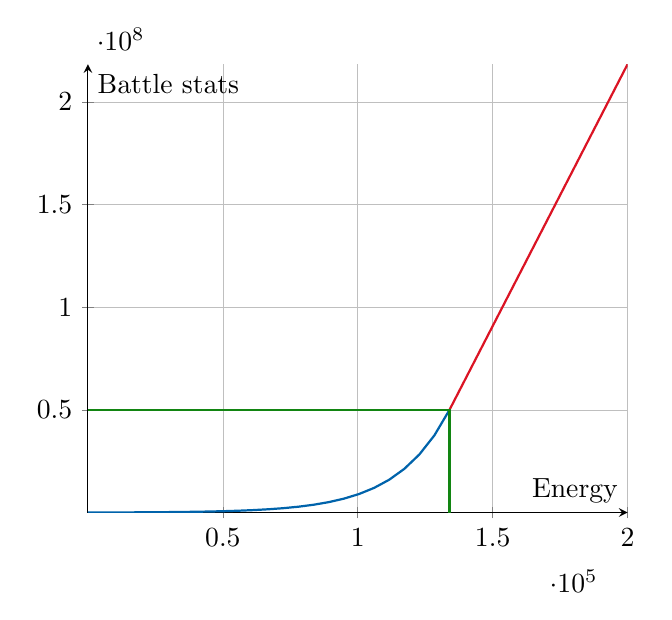
\begin{tikzpicture}
        \begin{axis}[
            % xmin=0,xmax=5000000,
            % ymin=0,ymax=100000000,
            grid=both,
            grid style={line width=.1pt, draw=gray!10},
            major grid style={line width=.2pt,draw=gray!50},
            axis lines=middle,
            % minor tick num=4,
            % ticks=none,
            ylabel=Battle stats,
            xlabel=Energy
        ]

           \def\alpha{0.0000509798};
           \def\beta{2.7561943022};
           \def\Ec{133988.1087149439};
           \def\Sc{50000000};
           \addplot[myblue, domain=0:\Ec, thick]{ \beta * (exp(\alpha * x) - 1) / \alpha };
           \addplot[myred, domain=\Ec:200000, thick]{ (\alpha * \Sc + \beta) * (x - \Ec) + \Sc };
           \draw[mygreen, thick] (axis cs:0,\Sc) -- (axis cs:\Ec,\Sc) -- (axis cs:\Ec,0);
           \end{axis}
    \end{tikzpicture}

    \caption{Battle stats as a function of energy for $\happy = 5000$, $\gym = 7.3$ and $\bonus= 15\%$}
    \label{fig:example}
\end{figure}

\subsection{Prediction formula}
In this section we are now interested at making a prediction of the energy needed $\Delta E$ to reach $\Sf$ from $\Si$:

\begin{equation}
    \Delta E = E(\Sf) - E(\Si)
    \label{eq:dE-definition}
\end{equation}
For this we need to anaylse the 3 cases:
\begin{enumerate}
    \item Before cap: $\Si < \Sc$ and $\Sf < \Sc$
    \item After cap: $\Si > \Sc$ and $\Sf > \Sc$
    \item Passing cap: $\Si < \Sc$ and $\Sf > \Sc$
\end{enumerate}
\subsubsection{Before cap: $\Si < \Sc$ and $\Sf < \Sc$}
Injecting eq.\eqref{eq:bs-bc-diff} in eq.\eqref{eq:dE-definition} gives
\begin{equation}
    \Delta E = \frac{1}{\alpha} \ln\left( \frac{1 + \alpha\Sf/\beta}{1 + \alpha\Si/\beta} \right)\\
\end{equation}

\subsubsection{After cap: $\Si > \Sc$ and $\Sf > \Sc$}
Injecting the linear relationship eq.\eqref{eq:bs-bc-diff-k} in eq.\eqref{eq:dE-definition} gives
\begin{equation}
    \Delta E = \frac{\Sf - \Si}{\alpha \Sc + \beta}
\end{equation}

\subsubsection{Passing cap: $\Si < \Sc$ and $\Sf > \Sc$}
In this last case both exponential and linear regime have to be taken into account.
We can decompose $\Delta E$ in two, the part needed to reach cap $\Delta E_\text{bc}$ (before cap) an the part in the linear regime $\Delta E_\text{ac}$ (after cap). $\Sc$ behing the frontiere between both, it plays the role of $\Sf$ for the exponential part and $\Si$ for the linear one. It reads:
\begin{equation}
    \begin{aligned}
        \Delta E = \Delta E_\text{bc} + \Delta E_\text{ac} = \frac{1}{\alpha} \ln\left( \frac{1 + \alpha\Sc/\beta}{1 + \alpha\Si/\beta} \right) + \frac{\Sf - \Sc}{\alpha \Sc + \beta}
    \end{aligned}
\end{equation}
\subsubsection{Generalized formula}
We can account for the three cases above in a single generalized equation\footnote{Mathematicians will not see the point, programmers will love it.}:
\begin{equation}
    \boxed{\Delta E = \underbrace{\frac{1}{\alpha} \ln\left( \frac{1 + \alpha\min(\Sc, \Sf)/\beta}{1 + \alpha\min(\Sc, \Si)/\beta} \right)}_\text{Before cap} + \underbrace{\frac{\max(\Sc, \Sf) - \max(\Sc, \Si)}{\alpha \Sc + \beta}}_\text{After cap}}
    \label{eq:de-s-general}
\end{equation}
where $\Delta E$ is the energy needed to reach $\Sf$ battle stats from $\Si$.

\section{Parametrical analysis}
\begin{center}
\color{myred}\bf DRAFT...
\end{center}

\subsection{The parameters}
With eq.\label{eq:de-s-general} it is now possible to quantify the impact of each state variables: $\happy$, $\gym$, $\bonus$ and the energy needed to acheive a battle stats goal.

\subsubsection{Effectiveness function}
We define an effectiveness function $\Ef(\happy, \gym, \bonus)$ that will return a number between 0 and 1 quantifying the effectiveness of the state variables to reach a battle stats goal. It is computed with respect to the energy needed to reach this goal ($\Delta E$) compared to the minimum possible $\Delta E^*$ ({\it i.e.} corresponding to $\happy_\text{max}, \gym_\text{max}, \bonus_\text{max}$).
\begin{equation}
    \Ef(\happy, \gym, \bonus) = \frac{\Delta E^*}{\Delta E}
\end{equation}

\subsubsection{Reaching stats cap}
In this case we set the goal to be reaching stats cap from 0 ($\Sf =\Sc$ and $\Si = 0$). Thus we have:
\begin{equation}
    \Ef(\happy, \gym, \bonus) = \frac{ \ln\left( 1 + \alpha_\text{max}\Sc/\beta_\text{max} \right) }{ \ln\left( 1 + \alpha\Sc/\beta \right) }
\end{equation}
where $\alpha$ and $\beta$ depend on $\happy, \gym, \bonus$.

\section{TODO}
\begin{itemize}
    \item find out why to quantify which from $\happy, \gym$ and $\bonus$ in pacts the most and when
    \item add a time / energy conversion
    \item Happy jumps and books...
    \item find out what torn's community wants to know
\end{itemize}

\end{document}
